\documentclass{article}
\usepackage{graphicx} 
\usepackage[dutch]{babel}
\usepackage{hyperref}
\usepackage{textcomp}
\begin{document}
\sffamily
\begin{titlepage}
  \centering
    \vfill
    {\bfseries\Huge
      Persoonlijke Verslag Tinlab Machine Learning \\
        \vskip2cm
      }
      {\bfseries\Large
        Raber Ahmad\\
      }
      {
        \bfseries\normalsize
        0921954\\
        \vskip1cm
        \today\\
    }    
    \vfill
    
\includegraphics[width=4cm]{logohr.png} % also works with logo.pdf
    \vfill
    \vfill
\end{titlepage}
\newpage
\tableofcontents
\newpage

\section{Inleiding}

Dit persoonlijke verslag dient als een samenvatting van alle informatie die is vergaard tijdens de Tinlab Machine Learning. Per onderwerp zal ruim/voldoende worden behandeld zodat dit document ook als een dictaat kan dienen voor je zelf.

\section{Introductie Machine learning}

\subsection{Wat is AI?}

Wanneer je je zelf afvraagt wat AI eigenlijk is, dan kun je dat op 2 manieren beantwoorden. Je kunt het beantwoorden met een wetenschappelijke doel maar ook met een technische doel. 
\\\\
Als technische doel wordt AI vaak gebruikt om problemen in de wereld op te lossen. Hierbij kun je denken aan Autonoom rijden en/of advertentie zo precies mogelijk te kunnen personaliseren zodat een product misschien meer wordt verkocht.
\\\\
Bij het wetenschappelijke doel wordt er meer gekeken naar de theorie achter AI. Er wordt bijvoorbeeld gekeken naar verschillende soorten Intelligentie, zoekmethodes en regelsystemen.

\subsection{Afkomst van AI}

Wanneer iemand aan AI denkt dan is het eerste wat er in je opkomt zijn robots die zich als een mens gedragen. AI komt eigenlijk uit verschillende takken van de wetenschap. Je kunt denken aan Biologie, Wiskunde, Filosofie en Computer Engineering. In 350BC formuleerde Aristotle bijvoorbeeld verschillende stijlen van redeneren daaruit konden conclusies uit worden getrokken. Aristotle was een filosoof\cite{aris}. Tot de dag van vandaag proberen wetenschappers verschillende technieken van AI te verbeteren iets wat al in 350BC is begonnen.

\subsubsection{Neurowetenschappen}

Het menselijk brein heeft ongeveer 100 miljard neuronen. Deze neuronen zijn via dendrieten en axons aan elkaar verbonden. Neuronen zijn cellen die informatie verwerken en doorsturen via elektrische pulsen en of chemische signalen\cite{neuron}. Een neurale netwerk uit de informatica is dus geïnspireerd uit het menselijk brein.

\section{Agents}
Een agent is een computerprogramma die handelingen doet voor een gebruiker of een ander programma\cite{agent}. Een Agent kan bijvoorbeeld een automatische stofzuiger zijn die aan de hand van hardware en sensoren de vloer stofvrij houdt.
We kunnen verschillende Agents van elkaar onderscheiden je hebt bijvoorbeeld Intelligent Adents en Locical Agents. In de sectie hieronder gaan we het over beide hebben.

\subsection{Intelligent Agents}

Wanneer je Intelligent Agent letterlijk vertaald uit het engels dan krijg je als antwoord "Intelligente onderhandelaars"\cite{intelligent-agent}. Met andere woorden Intelligent agents zijn agents die zelf beslissingen kunnen maken en zelfstandig opdrachten kunnen uitvoeren.

\subsubsection{PEAS}

PEAS staat voor Performance, Environment, Actuators en Sensors. PEAS is een model die veel intelligent agents gebruiken. Stel we willen een automatische stofzuiger bouwen. Dan is het verstandig om bepaalde eigenschappen voor de agent te specificeren. We kunnen dit als het volgende doen voor een automatische stofzuiger.

\begin{itemize}
    \item Measure of performance: Efficiënt, Zo snel mogelijk, Niet in de weg zitten.
    \item Environment: Woonkamer, Slaapkamer, Meubels, Personen
    \item Actuators: Sturen, Rijden, Stoppen, Stofzuigen
    \item Sensors: Camera, Sonar?
\end{itemize}

\subsection{Zoek Strategieën}
Een strategie wordt gedefinieerd bij het uitzoeken van de volgorde voor node uitbreiding. Hierbij wordt er rekening gehouden met verschillende aspecten. In de lijst hieronder hebben we een aantal hiervan.

\begin{itemize}
    \item Volledigheid : Vind ik altijd een oplossing als die bestaat?
    \item Tijd complexiteit: Aantal gegenereerde en uitgebreide nodes.
    \item Ruimte complexiteit: Maximaal aantal nodes in het geheugen.
    \item optimaal: Vindt het altijd een voordeligste oplossing?
\end{itemize}

\subsubsection{Uninformed search strategies}
Uninformed search strategies gebruiken alleen de informatie uit het probleem omschrijving. Hieronder hebben we een lijst van verschillende Uniform search strategies. Deze algoritme weten helemaal niks en zijn op zoek naar de oplossing van hun probleem. Zodra deze hun goal hebben gevonden geven ze een succes terug\cite{uss}.

\begin{itemize}
    \item Breadth First: Bij deze algoritme word er in de breedte gezocht.
    \item Depth-first: Hier zoekt hij altijd de diepte in.
    \item depth-limited: Lijkt heel erg veel op depth-first maar dan kun je er een limiet aan geven.
    \item Iterative Deeping: Wanneer depth-limited zijn limiet heeft bereikt dan kan hij die niet vergroten. Bij deze algoritme is het wel mogelijk.
    \item Uniform-cost: Meest optimale.
\end{itemize}

\begin{figure}[h!]
\centering
\begin{minipage}{.45\linewidth}
  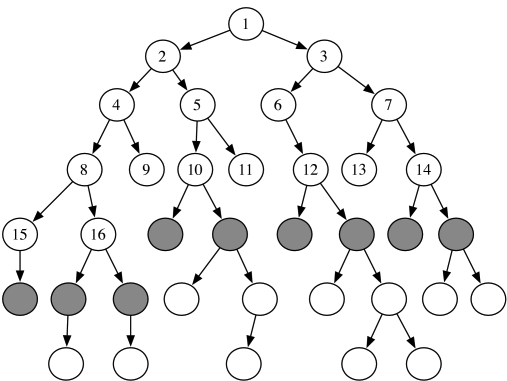
\includegraphics[width=\linewidth]{brd.png}
  \caption{Breadth-First}
  \label{Breadth-First}
\end{minipage}
\hspace{.05\linewidth}
\begin{minipage}{.45\linewidth}
  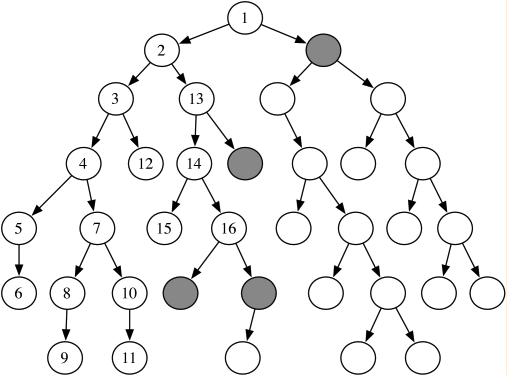
\includegraphics[width=\linewidth]{dept.png}
  \caption{Depth-first}
  \label{Depth-first}
\end{minipage}
\end{figure}

\subsection{Logica}
Logica 's zijn formele talen voor het representeren van informatie waarop conclusies over getrokken kunnen worden. In het eerst jaar van de opleiding technische informatica hebben we het vak propositie logica gehad. Veel van deze stof komt ook daadwerkelijk weer terug in machine learning. Voor meer informatie verwijs ik me zelf naar het dictaat logica van Wessel Oele\cite{logica}.

\begin{itemize}
    \item Logische constanten: true, false
    \item Propositie symbolen: P, Q, S, ... (atomic sentences)
    \item \land = And - Conjunctie$
    \item \vee  = Or - Disjunctie$
    \item \rightarrow = Impliceert - Implicatie$
    \item \leftrightarrow   = is equivalent - bi conditioneel$
    \item \neg  = Niet - Negatie$
\end{itemize}



\section{Uncertainty}
Zoals we eerder in dit document hebben beschreven, is AI geïnspireerd uit het menselijk brein. Dat betekend dat we in theorie ook misschien wel een persoon kunnen nabouwen die zijn eigen handelingen zelfstandig kan doen. 
\\\\
Wanneer we als mens buiten op straat lopen of in de auto zitten dan doen we eigenlijk wat ons is aangeleerd. We hebben leren lopen en de meeste hebben ook leren autorijden. Maar de vraag is, hoe wordt er gehandeld op bijzondere situaties? Hoe zouden wij reageren als we een ongeluk met een ander voertuig konden vermijden maar dat je daarnaast tegen een persoon aan zou rijden? En hoe zou een AI robot dat precies doen? Dit zijn allemaal zaken die we met AI heel moeilijk hebben. Er kan zoveel mogelijk getraind worden op bepaalde punten maar 1 bijzonder moment kan een drastische verandering geven aan de handelingen van een computer.


\section{Data Mining}
Data Mining houdt zich bezig met vinden van verbanden uit een grote dataset\cite{datamining}. Het doel ervan is om aan de hand van data die je in het verleden hebt gehad voorspellingen kunt doen voor de toekomst. Data Mining kan voor een bedrijf heel nuttig zijn. Zo kun je bijvoorbeeld advertenties personaliseren. Op sommige momenten kan het zo zijn dat je een advertentie krijgt voordat je er überhaupt over hebt nagedacht. Zo kreeg bijvoorbeeld een meisje advertenties van babykleding voordat ze zelf wist dat ze zwanger was\cite{preg}. Dit werd door middel van datamining voorspeld aan de hand van artikelen die ze eerder had gekocht.

\subsection{Tasks}

Data mining tasks kunnen in 2 groepen worden verdeeld gebaseerd op wat voor taak hij probeert te bereiken\cite{tasks}. De 2 groepen zijn descriptive tasks en predictive tasks.
\begin{itemize}
    \item Descriptive: Eigenschappen van de data beschrijven
    \item Predictive: Voorspellingen van nieuwe datasets
\end{itemize}
Verder Hebben beide groepen ook meerdere data mining tasks. Deze zijn classification, prediction, time-series analysis, association, clustering en summarization. Hieronder ziet u een diagram waar alles bij hoort.

\begin{figure}[h!]
  \centering
  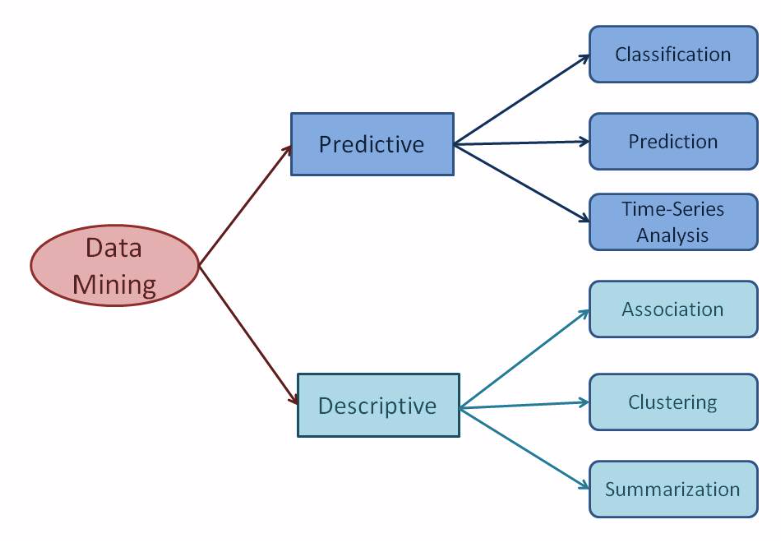
\includegraphics[scale=0.3]{tasks.png}
  \caption{Data mining tasks}
\end{figure}

\newpage
\section{Training methodes}
De 4 meest gebruikte training methodes zijn\cite{lm}.
\begin{itemize}
    \item Supervised learning
    \item Unsupervised learnging
    \item Semi supervised learning
    \item Reinforcment learning
\end{itemize}
Alle 4 methodes worden in bepaalde sectoren gebruikt. Je kunt hierbij denken aan spam detectie en of autonome rijden. Hieronder zien een een overzicht.
\begin{figure}[h!]
  \centering
  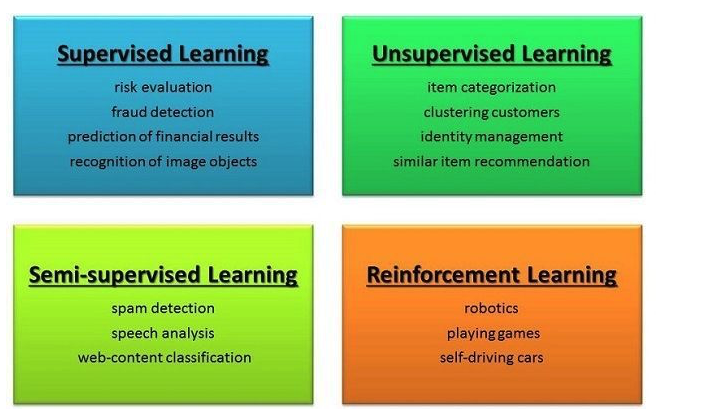
\includegraphics[scale=0.35]{lm.png}
  \caption{Learning methodes}
\end{figure}

\paragraph{Supervised learning}

Bij supervised learning wordt er daadwerkelijk gekeken naar de input met de correcte outputs. Alle data die supervised learning gebruikt moet gelabeld zijn. Typische cases voor supervised learning is herkennen van objecten of herkennen van fraude.
\paragraph{Unsupervised learning}
Hier leert de algoritme zich met onbekende data te trainen om zo patronen en de structuur van de data te herkennen. Dit word gebruikt bij bijvoorbeeld identiteit management of product categorieën.

\paragraph{Semi-Supervised Learning}
Bij semi-supervised word er gebruikt gemaakt van zowel bekende als onbekende data. Een klein deel van de data is bekend en een heel groot deel is onbekend. Dit wordt gebruikt bijvoorbeeld voor spam detectie in je mail.
\paragraph{Reinforcement Learning}
Bij reinforecment learning wordt er gebruikt gemaakt van trial-and-error. Dit betekend dat een systeem na heel veel oefenen zijn gewenste resultaat kan krijgen.
\section{Ethische verantwoording}
AI maakt het leven van heel veel personen makkelijk. Wanneer je je mail checkt dan checkt je mail server voor spam e-mails. Of wanneer je op vakantie gaat met het vliegtuig dan krijgt de piloot hulp van de automatische piloot. Zo kun je met een gerust hart op vakantie. 
\\\\
Naast heel veel goeds zijn er ook personen die hier misbruik van maken. Zo zijn er bijvoorbeeld bedrijven die jou data verzamelen en doorverkopen aan derde partijen. Al je foto 's die worden geüpload op het internet worden eerst door een filter heen gehaald en alles wordt gescand. 
\\\\
Daarom ben ik het niet mee eens hoe bedrijven zomaar al je data verzamelen en niemand weet wat er mee wordt gedaan. De main punt van het verzamelen van data is om deze zo goed mogelijk te analyseren en zo persoonlijke advertenties te zien krijgt. Als kun je bijvoorbeeld op Google naar een specifiek product zoeken en wanneer je een uur later op Instagram aan het scrollen bent dan zie je dit product ook terug bij de advertenties. Zoals ik eerder al had aangegeven kreeg een tiener meisje zelfs advertenties voor baby kleding nog voordat ze zelf wist dat ze zwanger was. Zo ver kan machine learning daadwerkelijk ook gaan om jou alleen persoonlijke advertenties te geven. Daar ben ik het niet mee eens en ik vind dat daar nog strengere regels ervoor moeten komen.
\section{Boekenclub}
Dit waren de taken die onder de boekenclubleiders waren verdeeld. Verder staan alle documenten te vinden in de map van de boekenclub.
\begin{itemize}
    \item Kirty: Maakte vooraf presentatie en hield notulen bij
    \item Sarah: Heeft samenvatting van SAT-Solvers gemaakt.
    \item Raber: Hield notulen bij en maakte samenvatting van DL redundantie
    \item Kaan : Was de spreker tijdens de boekenclub en maakte samenvatting van DL redundantie
\end{itemize}

\newpage
\begin{thebibliography}{}
\bibitem{aris}
Aristoteles. (2019, March 27). Retrieved June 19, 2019, from https://nl.wikipedia.org/wiki/Aristoteles
\bibitem{neuron}
How does a neuron work? (2013, November 13). Retrieved June 19, 2019, from https://www.wingsforlife.com/en/latest/how-does-a-neuron-work-562/
\bibitem{agent}
Software agent. (2019, May 11). Retrieved June 21, 2019, from https://en.wikipedia.org/wiki/Software\_agent
\bibitem{intelligent-agent}
Ede, J. V. (2007, August 22). Wat zijn Intelligent Agents? Retrieved June 22, 2019, from https://www.logistiek.nl/supply-chain/artikel/2007/08/wat-zijn-intelligent-agents-10133484
\bibitem{uss}
Artificial Intelligence 2E. (n.d.). Retrieved June 25, 2019, from https://artint.info/2e/html/ArtInt2e.Ch3.S5.html

\bibitem{logica}
W., Oele. (2016). Logica. Logica. Retrieved June 28, 2019, from https://med.hr.nl/oelew/logica/logica.pdf.
\bibitem{datamining}
Tuil, K. V. (2011, August 26). Wat is datamining? Retrieved June 28, 2019, from https://computerworld.nl/business-intelligence/74941-wat-is-datamining
\bibitem{preg}
Hill, K. (2016, March 31). How Target Figured Out A Teen Girl Was Pregnant Before Her Father Did. Retrieved June 29, 2019, from https://www.forbes.com/sites/kashmirhill/2012/02/16/how-target-figured-out-a-teen-girl-was-pregnant-before-her-father-did/#2392e0196668
\bibitem{tasks}
Wideskills. (n.d.). Retrieved June 30, 2019, from https://www.wideskills.com/data-mining-tutorial/05-data-mining-tasks
\bibitem{lm}
User, S. (2017, November 14). Machine Learning – Existing Applications. Retrieved July 1, 2019, from https://www.apriorit.com/dev-blog/472-machine-learning-applications
\end{thebibliography}{}
\end{document}


